\section{Theory Police}
The concept of Collective Intelligence itself has been around for thousands of years since people work, make decisions, and collaborate together in the form of families and communities. However, with the increasing advancement, spreading and adoption of information technologies and Internet, the idea of collective intelligence changes dramatically. In small scale, people are working together in labs, collaborating remotely through real time applications, and in other forms. Many study towards this direction look at how to improve the efficiency of information sharing, how to tranform implicit knowledge into explicit one, and how to reach the goal of problem-solving or product creation more effectively for the group as a whole. In large scale examples of collective intelligence, people look at crowdsourcing in differnet domains like finance, citizen science and knowledge creation. Even though collective intelligence at scale is heavily focusing on the crowdsourcing, we do not have a integrated definition towards the meaning of crowdsourcing. So in the theory police part, first, we are examining the integrated definition of it.

\subsection{Integrated Definition of Crowdsourcing}
The work we refer to is called Towards an Integrated Crowdsourcing defnition by Enrique Estelles-Aroles and Fernando Gonzalez-Ladron-de-Guevara. The problem they see in the field is that the diversity of crowdsourcing applications leads to the blurring of the limits of crowdsourcing, which could be identified virtually with any type of internet-based collaborative activity. Thus, The paper used literature review as research method to find an validated exhaustive definition of crowdsourcing. By doing so, first, it follows the Tatarkiewicz's approach to include all the paper that relate to crowdsourcing and all the elements whose characteristics differentiate crowdsourcing from other collaborative activities based on ICT. Second, it borrows Vukovic and Aliabarian's view to check the validity of the definition. In the end, it presents its findings of three main elements in the definition of crowdsourcing which are crowd, initiator and process. Crowd has three characterisitcs, which are who forms it; what it has to do; and what it gets in return. For initiator, it has to answer two question: who it is; and what they get in return for the work of the crowd. For process, the type of process; the type of call used; and the medium used are the three main features to identify\cite{theorypolice1}.

\subsection{Differences With Distributed Cognition}
We naturally link Collective Intelligence theory with Distributed Cognition theory for the similarities they share. For example, they both study groups; they both have a specific goal to achieve: either problem-solving or product creation; and they all have three main elements in their theory: group of people, problems/goals and tools. But also they have significant differences to distinguish with each other.

First, they have different origin. Distributed Cognition is coming from psychology. It studies how groups coordinate their behaviors with each other. It treats group work as cognitive problems because the system exhibits purposeful behaviors in problem solving and information processing\cite{dcog}. Collective Intelligence is more commonly found in management science and organizational study. 

Second, Distribted Cognition could be used to discover social and cultural dimensions of work, relating these back to system development and HCI. However, the relationship between Collective Intelligence with HCI is not as directly applied as DCog with HCI.

Third, the sizes of groups on which these two theories study are different from each other. Collective Intelligence has a broader scope of groups, which ranges from small 2-5 member groups to thousands people from crowdsourcing applications. However, DCog is applied in much smaller groups than Collective Intelligence.

Forth, Distributed Cognition is a more closed system than Collective Intelligence. The following figure shows that DCog system has its input and output, and in between there are human-computer representations and the processes between them. Like cognitive system, Dcog has
its information processing activities but with both human minds and computers. But for Collective Intelligence, we do not see this clear and closed system developed yet.

\begin{figure}[!h]
\centering
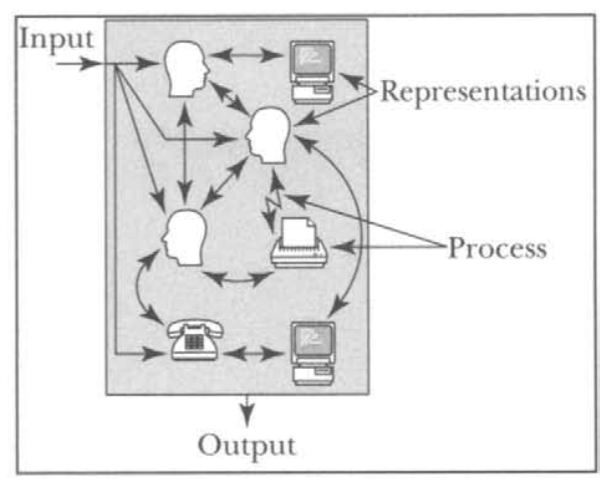
\includegraphics[width=0.9\columnwidth]{figure/DCog}
\caption{Distributed Cognition System}
\label{fig:Dcog}
\end{figure}



